\documentclass{article}
\usepackage[utf8]{inputenc}

\usepackage[letterpaper, margin=1in]{geometry}
\title{Generative Adversarial Networks}
\author{Justin Zhang}
\date{July 2017}

\usepackage{natbib}
\usepackage{graphicx}
\usepackage{epigraph}
\usepackage{float}

\begin{document}

\maketitle

\section{Introduction}
    Generative Adversarial Networks (GANs) are a seminal type of generative model, introduced in 2014 by the University of Montreal. GANs have been heavily used in various generative tasks with impressive results. GANs are most actively used for image generation tasks: plain image generation, image inpainting, super-resolution image generation, and text-to-image. However, they are beginning to see some use in other types of inputs (e.g. audio, video, etc). Since GAN's first release, there have been multiple iterations on different types of GANs; here, we'll cover the basics only.
\section{Intuition}
    GANs consist of two neural networks: the generator and the discriminator. The generator is tasked with generating fake samples from random noise. The discriminator is tasked with distinguishing fake samples with real ones (from the dataset).
    \begin{center}
    \begin{figure}[H]
        \centerline{\includegraphics[scale=0.25]{gan.png}}
        \caption{The GAN pipeline.}
        \label{fig:gan}
    \end{figure}
    \end{center}
    In this way, the two networks play a game of cat-and-mouse; they each try to beat the other. Thoughout training, the goal is to have both networks simultaneously improve: the generator increasingly generates more convincing images to fool the discriminator, and the discriminator becomes better at separating real and fake samples as a result.
\section{Training specifics}
    With regards to images, usually deep convolutional layers are used, for both the discriminator and the generator.
    \begin{figure}[H]
        \centerline{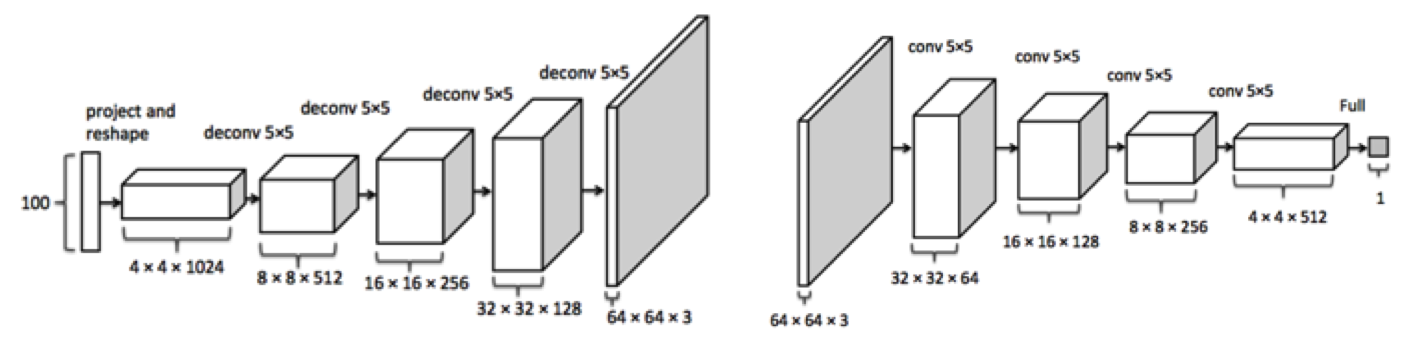
\includegraphics[scale=0.5]{dcgan.png}}
        \caption{The DCGAN pipeline.}
        \label{fig:dcgan}
    \end{figure}
    Here, deconvolutional layers are used in the generator to produce the target $64$ by $64$ image. This image is then fed into the discriminator for classification.
    
    A typical training pipeline would be to randomly initialize the two networks. Then, we would iterate over the dataset. At each iteration, we would generate the batch size number of fake images from the generator, so that we would have an equal number of fake and real images. Then, we could train the discriminator on these images with a binary cross-entropy loss. Finally, imagine the generator and discriminator to be one large network, going from noise (via uniform or gaussian) as input into the generator and discriminator to the binary output. In the perspective of the generator, we want to output the incorrect labels (i.e. always $1$, the output is the probability of the input to the discriminator being a real image) in this concatenated network. In this way, we can freeze the discriminator weights and flow the gradients through it to train the generator. We can then repeat this for each batch, over a number of epochs, as per usual.
    
    Note that GANs are notoriously difficult to train. This is because GANs are highly unstable; in order to train correctly, we need the generator and discriminator to be roughly on equal levels throughout the training process. If the discriminator overpowers the generator, there will be little gradient for the generator to learn upon; vice-versa, and we run into \textit{mode collapse}, where the generator produces outputs with extremely low variety.
    

\section{Applications}
    GANs are not yet frequently used in applications, especially at the high school level -- so finding a decent (novel) application for them could be a great project idea.
    
    Here are some examples:

    \begin{figure}[H]
        \centerline{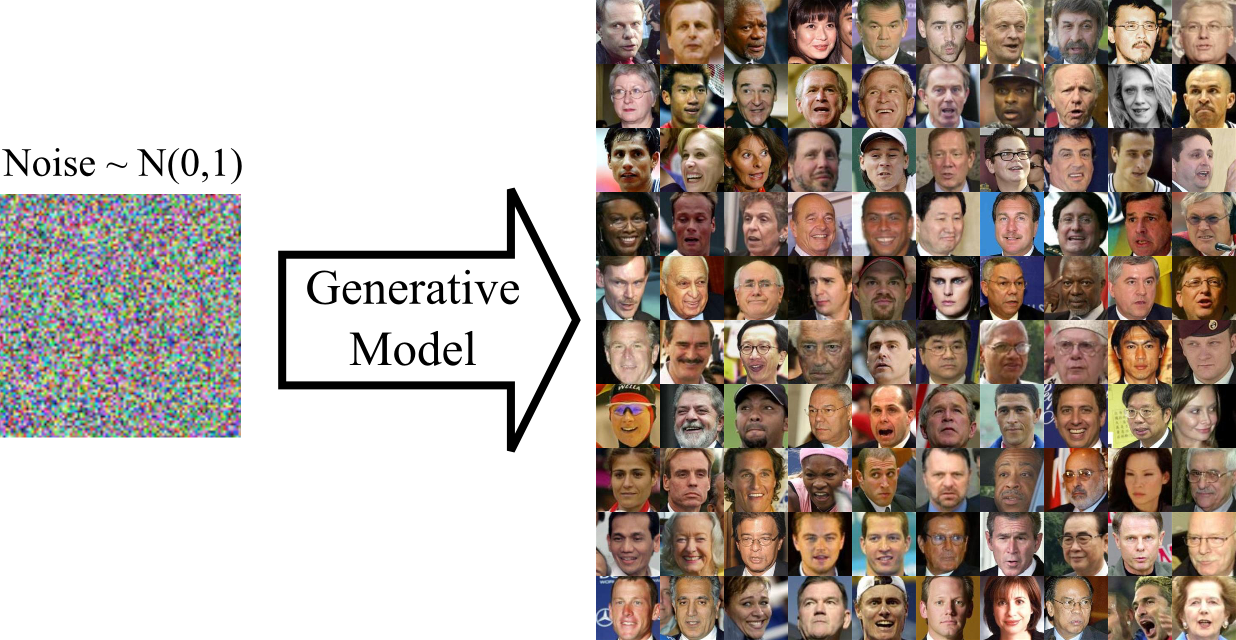
\includegraphics[scale=0.3]{image_generation.png}}
        \caption{Image generation.}
        \label{fig:image_generation}
    \end{figure}
    
    This has been done with a variety of GANs (e.g. Wasserstein GAN), and can be done (with limited success) with vanilla GANs. There are also architectures that convert a caption to an image, with remarkable success (e.g. StackGAN++).
    
    
    \begin{figure}[H]
        \centerline{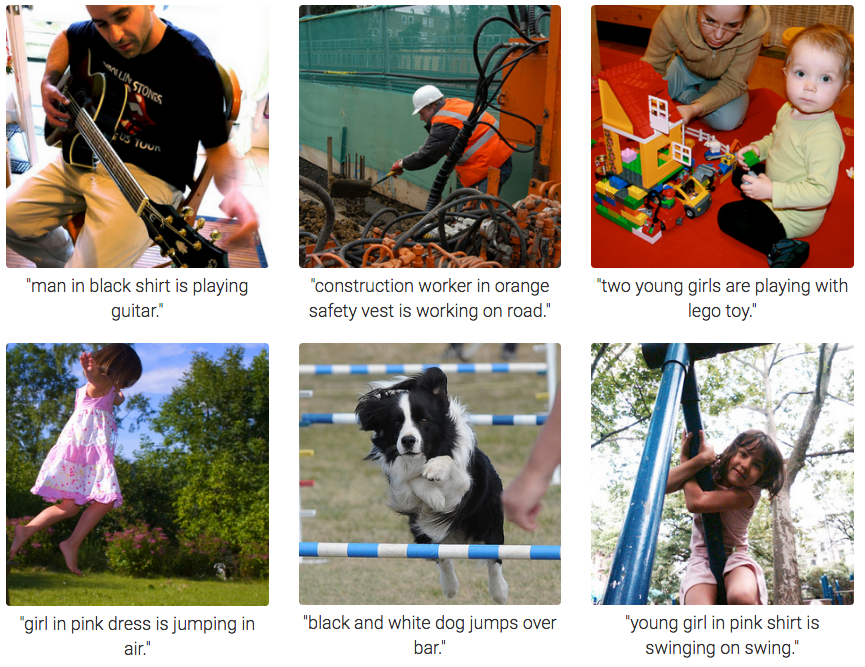
\includegraphics[scale=0.3]{caption_generation.png}}
        \caption{Caption generation.}
        \label{fig:caption_generation}
    \end{figure}
    
    Conditional GANs (as well as RNNs) have been used, to much success, for this task.
    
    
    
    \begin{figure}[H]
        \centerline{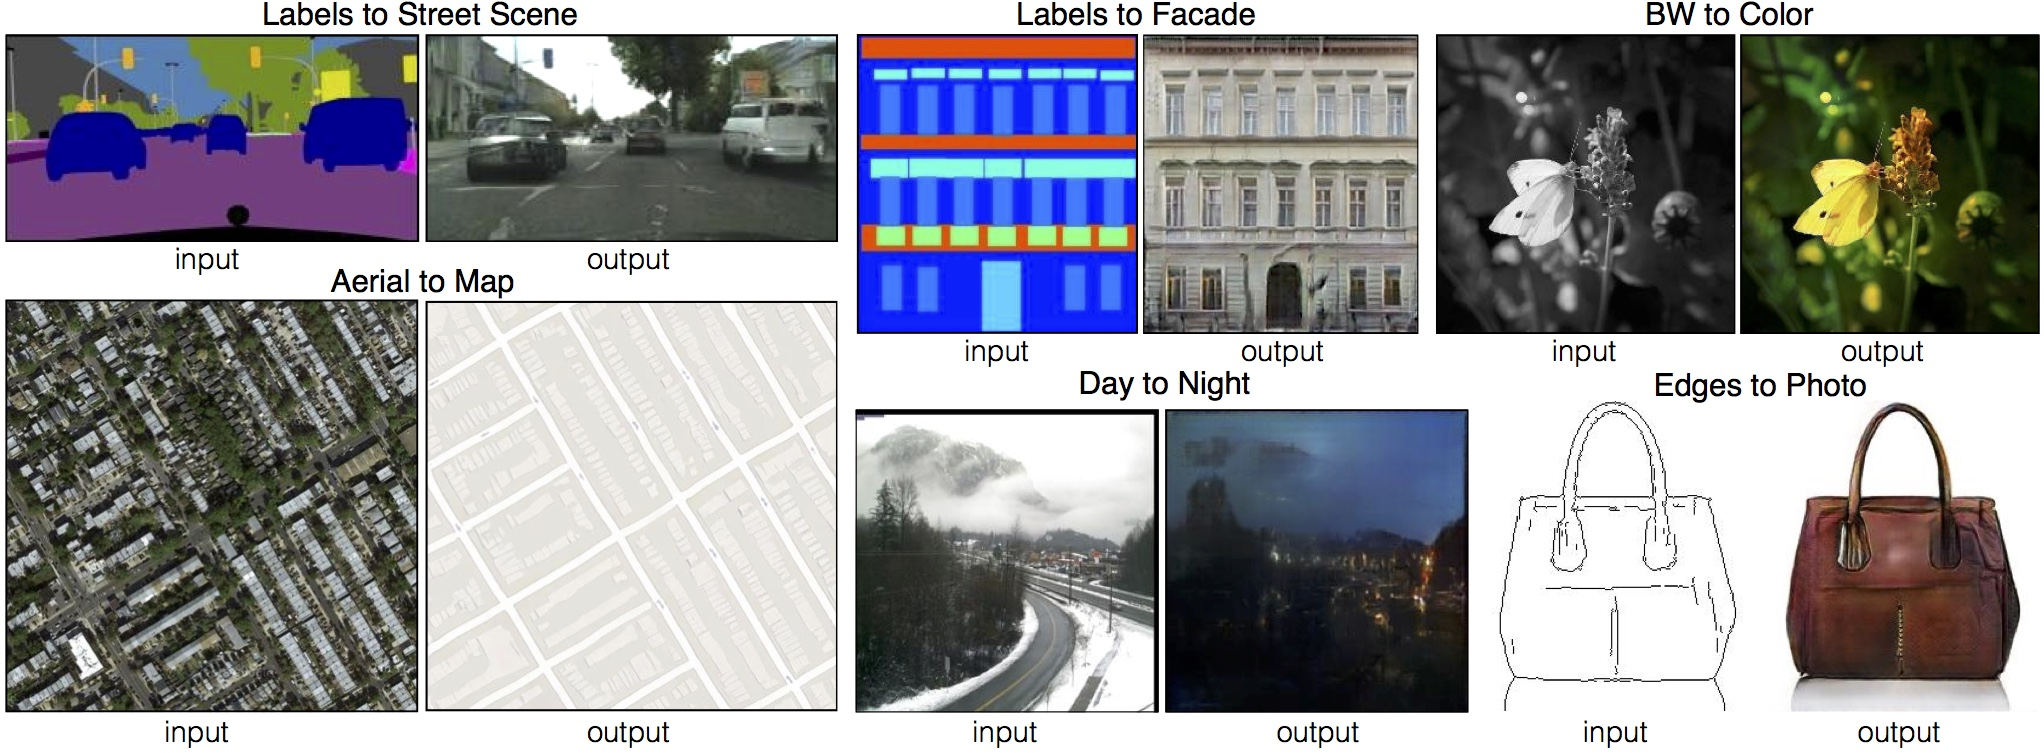
\includegraphics[scale=0.2]{pix2pix.jpg}}
        \caption{Image mapping.}
        \label{fig:mapping}
    \end{figure}
    
    Two prominent networks for this task are the pix2pix network (Conditional GAN) and the CycleGAN. The results, as you can see, are quite impressive, and can be extended to a variety of image-based tasks.
    
    \begin{figure}[H]
        \centerline{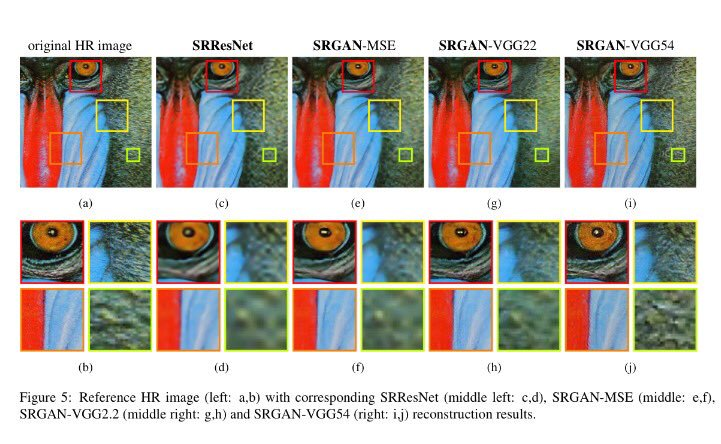
\includegraphics[scale=0.4]{superres.jpg}}
        \caption{Super-resolution.}
        \label{fig:super-resolution}
    \end{figure}
    
    GANs have been used in the task of super-resolution, interpolating finer texture details that are lost in a low-res image. The most prominent architecture for this task is the SRGAN. The SRGAN has been used to moderate success (though MOS scores are subjective and difficult to validate). 
    
    
\section{Math}
    The gradient expression we train the discriminator on is as follows:
    $$\nabla \frac{1}{m} \sum_{i=1}^m [\log D(x_i) + \log(1-D(G(z_i))]$$
    where $x$ is the real data in a given batch, $z$ is the noise for the generator for the given batch, $D$ is the discriminator function, and $G$ is the generator. We want to maximize this expression. The first expression in the summation, $\log D(x_i)$, corresponds to the discriminator output on real data; we clearly want to maximize this probability. The second is a bit more complicated: the $D(G(z_i))$ corresponds to the discriminator's probability estimate that the generated data is real. We want to minimize this, so we make the term $\log (1-D(G(z_i))$. If you haven't taken multivariable calculus yet, think about the $\nabla$ as a derivative; we simply want to move in the direction that maximizes the summation.
    
    The gradient expression we train the generator on is as follows:
    $$\nabla \frac{1}{m} \sum_{i=1}^m \log(1-D(G(z_i))$$
    We want to minimize this expression (i.e. we want to maximize $D(G(z_i))$, the probability of the generated data being real, as determined by the discriminator).
    
    
\section{CycleGAN}

    \begin{figure}[H]
        \centerline{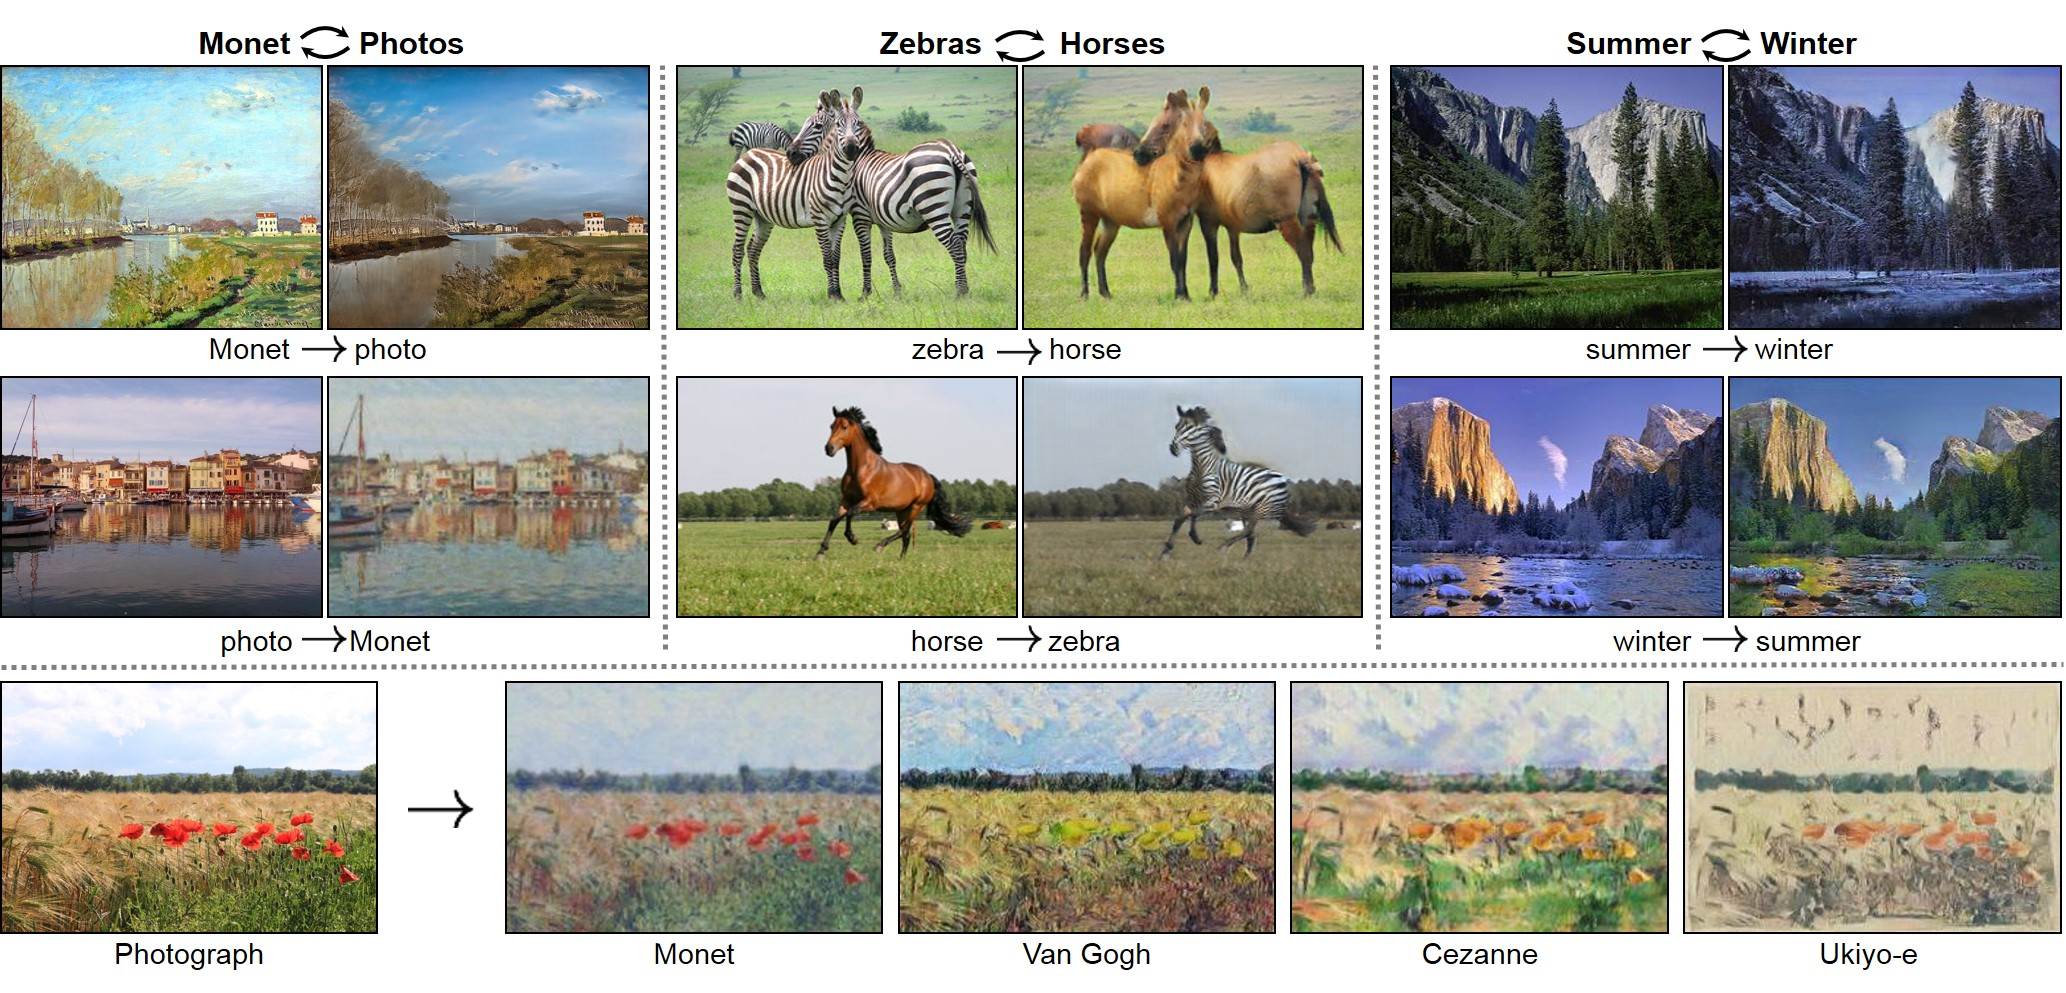
\includegraphics[scale=0.3]{cyclegan.jpg}}
        \caption{The CycleGAN.}
        \label{fig:cyclegan}
    \end{figure}

    The goal of the CycleGAN is to learn a mapping $G$ that translates a source domain $X$ to a target domain $Y$ given unpaired images.
    
    However, the problem of learning $G$ such that $G(X) \rightarrow Y$ is that the mapping $G$ is very under-constrained (in other words, there are many ways that $G$ can minimize loss of the dataset as a whole while producing qualitatively not-very-good individual images). The basic approach of the CycleGAN, thus, is to ensure \textit{cyclic consistency} by introducing an inverse mapping $F$ and a cyclic consistency loss that enforces $F(G(X)) \approx X$ and $G(F(Y)) \approx Y$.

    As usual, the loss for $G$ is $$min_G\,max_{D_Y} \log D_Y(x_i) + \log(1-D_Y(G(z_i))$$ An analogous loss is used for $F$.
    
    However, a new term is introduced for cyclic consistency: $$\lambda ||F(G(x)) - x||_1 + ||G(F(y)) - y||_1$$ The L1 norm was selected based on empirical data.
    
    The final loss, then, is the sum of these three individual losses.
    
    The CycleGAN's architecture is based on pix2pix's PatchGAN, which essentially uses a discriminator that classifies NxN patches. This helps to preserve smaller details, such as texture and style.
    
    The architecture was evaluated with both qualitative (Amazon Mechanical Turk) and quantitative (FCN) scores, and achieved state-of-the-art results (though it was still soundly defeated by pix2pix, which relies on \textit{paired} images).
    

    
\section{Conclusion}
    GANs are incredibly useful models; however, training them can be very difficult. GANs are continuously being improved to increase stability and to accommodate different types of input. Stay tuned for Nikhil's lecture next week on newer GANs!
    
    We hope to see more GAN projects in the coming months, and we're confident that there are many unexplored uses for them. 
    
    For more tips on training a GAN, see this link [https://github.com/soumith/ganhacks]. Seriously. It'll be useful.
    
    For an example of a GAN, see this link. [https://github.com/jacobgil/keras-dcgan/blob/master/dcgan.py]\\
    
\end{document}
